\documentclass[12pt,a4paper]{article}

% --- Page Layout -------------------------------------------------------------
\usepackage[a4paper, margin=0.8in, headheight=14pt]{geometry}

% --- Fonts (XeLaTeX) ---------------------------------------------------------
\usepackage{fontspec}
\usepackage{unicode-math}
\setmainfont{TeX Gyre Pagella}
\setmonofont[Scale=0.88]{TeX Gyre Cursor}
\setmathfont{Latin Modern Math}

% --- Packages ---------------------------------------------------------------
\usepackage{xcolor}
\usepackage{titlesec}
\usepackage{enumitem}
\usepackage{tabularx}
\usepackage{booktabs}
\usepackage{array}
\usepackage{amsmath}
\usepackage{tikz}
\usetikzlibrary{shapes.geometric, arrows.meta, positioning, calc, fit, decorations.pathreplacing, decorations.pathmorphing}
\usepackage{tcolorbox}
\tcbuselibrary{skins, breakable}
\usepackage{hyperref}
\usepackage{fancyhdr}
\usepackage{graphicx}
\usepackage{microtype}
\hyphenpenalty=10000
\exhyphenpenalty=10000
\sloppy
\usepackage{caption}
\usepackage{setspace}
\usepackage{multirow}
\usepackage{tocloft}

% --- Q&A helper --------------------------------------------------------------
\newcommand{\Q}[1]{\textbf{#1}\par\noindent\ignorespaces}

% --- Colour Palette ----------------------------------------------------------
\definecolor{myred}{RGB}{196,30,58}
\definecolor{mydark}{RGB}{30,30,50}
\definecolor{mygreen}{RGB}{14,120,80}
\definecolor{myteal}{RGB}{0,130,140}
\definecolor{myamber}{RGB}{180,100,0}
\definecolor{mypurple}{RGB}{100,30,160}
\definecolor{mygray}{RGB}{246,247,249}
\definecolor{mgframe}{RGB}{180,185,200}
\definecolor{watermark}{RGB}{145,150,170}
\definecolor{hdrred}{RGB}{250,232,235}
\definecolor{hdrgreen}{RGB}{220,244,233}
\definecolor{hdrteal}{RGB}{220,242,244}
\definecolor{hdramber}{RGB}{253,242,215}
\definecolor{hdrpurple}{RGB}{238,228,255}

% --- Section Formatting ------------------------------------------------------
\titleformat{\section}
  {\large\bfseries\color{myred}}{\thesection.}{0.5em}{}
  [\vspace{1pt}{\color{myred}\rule{\linewidth}{0.8pt}}]
\titleformat{\subsection}
  {\normalsize\bfseries\color{myteal}}{\thesubsection}{0.5em}{}
\titlespacing*{\section}{0pt}{18pt}{7pt}
\titlespacing*{\subsection}{0pt}{11pt}{4pt}

% --- Paragraph ---------------------------------------------------------------
\setlength{\parindent}{0pt}
\setlength{\parskip}{4pt}

% --- TOC Styling -------------------------------------------------------------
\renewcommand{\cfttoctitlefont}{\large\bfseries\color{myred}}
\renewcommand{\cftaftertoctitle}{\par\noindent{\color{myred}\rule{\linewidth}{0.8pt}}}
\setlength{\cftbeforetoctitleskip}{0pt}
\setlength{\cftaftertoctitleskip}{6pt}
\renewcommand{\cftsecfont}{\normalsize\bfseries\color{mydark}}
\renewcommand{\cftsecpagefont}{\normalsize\bfseries\color{mydark}}
\renewcommand{\cftsecleader}{\cftdotfill{\cftdotsep}}
\setlength{\cftbeforesecskip}{7pt}
\renewcommand{\cftsubsecfont}{\small\color{mydark}}
\renewcommand{\cftsubsecpagefont}{\small\color{mydark}}
\setlength{\cftbeforesubsecskip}{3pt}
\setlength{\cftsubsecindent}{1.4em}

% --- Table helpers -----------------------------------------------------------
\renewcommand{\arraystretch}{1.45}
\setlength{\tabcolsep}{6pt}
\newcolumntype{B}[1]{>{\small\bfseries\raggedright\arraybackslash}m{#1}}
\newcolumntype{Y}{>{\small\raggedright\arraybackslash}X}
\renewcommand{\tabularxcolumn}[1]{m{#1}}

% --- Header / Footer ---------------------------------------------------------
\pagestyle{fancy}
\fancyhf{}
\fancyhead[L]{\small\color{myred}\textbf{BS-PH101}\;\color{mydark}--- Physics-I}
\fancyhead[R]{\small\color{myteal}\textbf{Module 4 Notes}}
\fancyfoot[C]{\small\color{mydark}\thepage}
\fancyfoot[R]{\small\color{watermark}\textit{\copyright\ Biraj}}
\renewcommand{\headrulewidth}{0.5pt}
\renewcommand{\footrulewidth}{0.3pt}

% --- Hyperref ---------------------------------------------------------------
\hypersetup{
  colorlinks=true, linkcolor=myteal, urlcolor=myteal,
  pdfauthor={Biraj Sarkar},
  pdftitle={BS-PH101 --- Module 4 Notes}
}

% --- tcolorbox styles --------------------------------------------------------
\tcbset{
  tikzbox/.style={
    colback=mygray, colframe=mgframe, boxrule=0.6pt, arc=4pt,
    left=8pt, right=8pt, top=6pt, bottom=6pt,
    colbacktitle=mgframe, coltitle=mydark, fonttitle=\small\bfseries
  },
  defbox/.style={
    colback=hdrgreen, colframe=mygreen, boxrule=0.8pt, arc=4pt,
    left=9pt, right=9pt, top=6pt, bottom=6pt,
    colbacktitle=mygreen, coltitle=white, fonttitle=\small\bfseries
  },
  formulabox/.style={
    colback=hdrteal, colframe=myteal, boxrule=0.8pt, arc=4pt,
    left=9pt, right=9pt, top=7pt, bottom=7pt,
    colbacktitle=myteal, coltitle=white, fonttitle=\small\bfseries
  },
  examplebox/.style={
    colback=hdramber, colframe=myamber, boxrule=0.8pt, arc=4pt,
    left=9pt, right=9pt, top=6pt, bottom=6pt,
    colbacktitle=myamber, coltitle=white, fonttitle=\small\bfseries
  },
  masonbox/.style={
    colback=hdrpurple, colframe=mypurple, boxrule=0.8pt, arc=4pt,
    left=9pt, right=9pt, top=6pt, bottom=6pt,
    colbacktitle=mypurple, coltitle=white, fonttitle=\small\bfseries
  },
  exambox/.style={
    colback=hdrpurple, colframe=mypurple, boxrule=1pt, arc=5pt,
    left=10pt, right=10pt, top=8pt, bottom=8pt,
    colbacktitle=mypurple, coltitle=white, fonttitle=\bfseries,
    breakable, title after break={\textbf{Frequently Asked / Viva Questions (contd.)}}
  }
}
\tcbset{breakable}

% --- TikZ Styles -------------------------------------------------------------
\tikzset{
  block/.style={rectangle, draw=myteal, fill=hdrteal, text width=2.4cm, align=center, minimum height=0.95cm, font=\small, rounded corners=3pt, line width=0.7pt},
  redblock/.style={rectangle, draw=myred, fill=hdrred, text width=2.4cm, align=center, minimum height=0.95cm, font=\small, rounded corners=3pt, line width=0.7pt},
  arrow/.style={-Stealth, thick, color=mydark},
  redarrow/.style={-Stealth, thick, color=myred},
  line/.style={thick, color=mydark}
}

\begin{document}

% --- Title Page --------------------------------------------------------------
\begin{center}
  {\LARGE\bfseries\color{myred} BS-PH101 --- Physics-I}\\[5pt]
  {\normalsize\color{mydark} Semester I/II \quad$\bullet$\quad 3L:1T:0P \quad$\bullet$\quad 4 Credits}\\[3pt]
  {\normalsize\color{myteal}\textbf{Module 4 Comprehensive Exam Notes: Quantum Mechanics}}\\[3pt]
  {\small\color{mydark} CGEC \;$|$\; B.Tech ECE (2023--27) \;$|$\; \textit{Biraj Sarkar}}
\end{center}
\vspace{2pt}
\noindent{\color{myred}\rule{\linewidth}{1.5pt}}
\vspace{2pt}
\hypersetup{linkcolor=mydark}
\tableofcontents
\hypersetup{linkcolor=myteal}
\newpage

% =============================================================================
% SECTION 1: INADEQUACY OF CLASSICAL PHYSICS & BLACK BODY RADIATION
% =============================================================================
\section{Inadequacy of Classical Physics and Black Body Radiation}

\subsection{Failure of Classical Mechanics and Planck's Radiation Law}

Classical physics (Rayleigh-Jeans law $u(\nu)d\nu = \frac{8\pi \nu^2}{c^3} k_B T d\nu$) predicted that black body radiation energy density tends to infinity at short wavelengths ($\lambda \to 0$), known as the \textbf{Ultraviolet Catastrophe}.

\begin{tcolorbox}[defbox, title={\textbf{Planck's Quantum Hypothesis (1900)}}]
Black body cavity walls consist of atomic oscillators that absorb or emit electromagnetic radiation in discrete packets called \textbf{quanta} (photons) of energy:
\begin{equation}
E = n h \nu \quad (n = 1, 2, 3, \ldots)
\end{equation}
where $h = 6.626 \times 10^{-34}\text{ J}\cdot\text{s}$ is Planck's constant.
\end{tcolorbox}

\begin{tcolorbox}[formulabox, title={\textbf{Planck's Black Body Radiation Law Derivation}}]
Average energy of an oscillator $\langle E \rangle = \frac{\sum_{n=0}^\infty n h\nu \, e^{-n h\nu / k_B T}}{\sum_{n=0}^\infty e^{-n h\nu / k_B T}} = \frac{h\nu}{e^{h\nu / k_B T} - 1}$.
Multiplying by number of modes per unit volume $N(\nu)d\nu = \frac{8\pi \nu^2}{c^3} d\nu$:
\begin{equation}
u(\nu) d\nu = \frac{8\pi h \nu^3}{c^3} \frac{1}{e^{h\nu / k_B T} - 1} d\nu \iff u(\lambda) d\lambda = \frac{8\pi h c}{\lambda^5} \frac{1}{e^{hc / \lambda k_B T} - 1} d\lambda
\end{equation}
\end{tcolorbox}

\textbf{Deduction of Limiting Laws:}\par\noindent
\begin{itemize}[leftmargin=*, itemsep=3pt]
  \item \textbf{Rayleigh-Jeans Law (Long $\lambda$):} For $h\nu \ll k_B T$, $e^{h\nu/k_B T} - 1 \approx \frac{h\nu}{k_B T} \implies u(\nu)d\nu = \frac{8\pi \nu^2}{c^3} k_B T d\nu$.
  \item \textbf{Wien's Distribution Law (Short $\lambda$):} For $h\nu \gg k_B T$, $e^{h\nu/k_B T} - 1 \approx e^{h\nu/k_B T} \implies u(\lambda)d\lambda = \frac{8\pi hc}{\lambda^5} e^{-hc/\lambda k_B T} d\lambda$.
\end{itemize}

% =============================================================================
% SECTION 2: COMPTON EFFECT & MATTER WAVES
% =============================================================================
\section{Compton Effect, de Broglie Hypothesis, and Matter Waves}

\subsection{Compton Effect}

When a high-energy X-ray or $\gamma$-ray photon collides elastically with a stationary free electron, the scattered photon emerges with a longer wavelength ($\lambda' > \lambda$).

\begin{tcolorbox}[formulabox, title={\textbf{Derivation of Compton Shift Formula}}]
Applying conservation of relativistic energy and momentum during collision:
\begin{align}
\text{Energy Conservation: } & h\nu + m_0 c^2 = h\nu' + m c^2 \\[4pt]
\text{Momentum Conservation: } & \vec{p}_{\text{photon}} = \vec{p}'_{\text{photon}} + \vec{p}_{\text{electron}}
\end{align}
Eliminating electron velocity $v$ using $m = \frac{m_0}{\sqrt{1 - v^2/c^2}}$ yields the \textbf{Compton Shift Equation}:
\begin{equation}
\Delta \lambda = \lambda' - \lambda = \frac{h}{m_0 c} (1 - \cos\theta) = 2 \lambda_c \sin^2\left(\frac{\theta}{2}\right)
\end{equation}
where $\lambda_c = \frac{h}{m_0 c} = 0.02426\text{ \AA} = 2.426 \times 10^{-12}\text{ m}$ is the \textbf{Compton Wavelength}.
\end{tcolorbox}

\textbf{Key Characteristics of Compton Shift:}
\begin{itemize}[leftmargin=*, itemsep=2pt]
  \item $\Delta \lambda$ depends \textit{only} on scattering angle $\theta$, independent of incident wavelength or target material.
  \item Maximum shift occurs at $\theta = 180^\circ$ (backscattering): $\Delta \lambda_{\max} = \frac{2h}{m_0 c} = 0.0485\text{ \AA}$.
  \item Compton shift is absent for visible light because $\Delta\lambda \ll \lambda_{\text{visible}}$ is unresolvable.
\end{itemize}

\begin{tcolorbox}[tikzbox, title={Compton Scattering Geometry}]
\centering
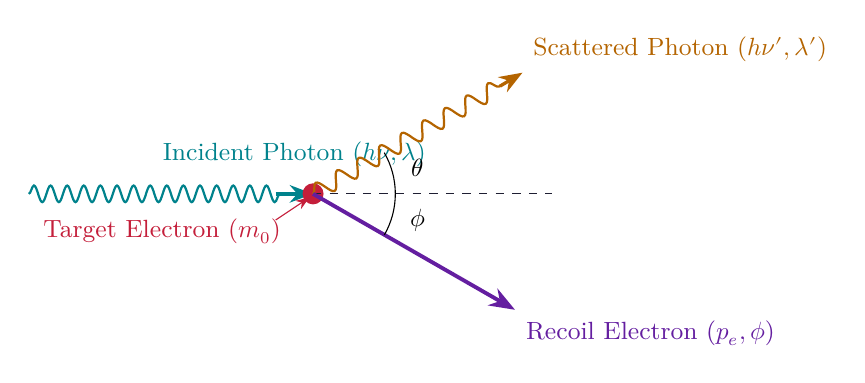
\begin{tikzpicture}[scale=0.95]
  % Incident Photon Wave
  \draw[thick, myteal, decorate, decoration={snake, segment length=6pt, amplitude=3pt}] (-3.8,0) -- (-0.4,0);
  \draw[-Stealth, line width=1.2pt, myteal] (-0.5,0) -- (0,0) node[midway, above=6pt] {\small Incident Photon ($h\nu, \lambda$)};
  
  % Target Electron
  \fill[myred] (0,0) circle (4pt);
  \node[myred, anchor=east] at (-0.3,-0.5) {\small Target Electron ($m_0$)};
  \draw[-Stealth, thin, myred] (-0.5,-0.35) -- (-0.05,-0.05);
  
  % Dashed baseline
  \draw[dashed, mydark] (0,0) -- (3.2,0);

  % Scattered Photon Wave
  \draw[thick, myamber, decorate, decoration={snake, segment length=9pt, amplitude=3pt}] (0,0) -- (2.6, 1.5);
  \draw[-Stealth, line width=1.2pt, myamber] (2.5, 1.44) -- (2.8, 1.62) node[above right] {\small Scattered Photon ($h\nu', \lambda'$)};
  \draw[thin] (1.1,0) arc (0:30:1.1);
  \node at (1.4,0.35) {\small $\theta$};
  
  % Recoil Electron
  \draw[-Stealth, line width=1.4pt, mypurple] (0,0) -- (2.7, -1.55) node[below right] {\small Recoil Electron ($p_e, \phi$)};
  \draw[thin] (1.1,0) arc (0:-30:1.1);
  \node at (1.4,-0.35) {\small $\phi$};
\end{tikzpicture}
\end{tcolorbox}

\subsection{de Broglie Hypothesis and Davisson-Germer Experiment}

\begin{tcolorbox}[defbox, title={\textbf{Definition: de Broglie Hypothesis}}]
Louis de Broglie (1924) proposed that moving matter particles exhibit wave properties with a wavelength ($\lambda$) inversely proportional to momentum ($p$):
\begin{equation}
\lambda = \frac{h}{p} = \frac{h}{m v} = \frac{h}{\sqrt{2m E}} = \frac{h}{\sqrt{2m q V}}
\end{equation}
For an electron accelerated through potential $V$ volts:
\begin{equation}
\lambda_e = \frac{12.27}{\sqrt{V}} \text{ \AA}
\end{equation}
\end{tcolorbox}

\textbf{Davisson-Germer Experiment:} Accelerated electrons at $V = 54\text{ V}$ onto a Nickel crystal target observed a pronounced scattering peak at angle $\phi = 50^\circ$.
Bragg diffraction angle $\theta = 90^\circ - \phi/2 = 65^\circ$.
\begin{equation}
\lambda_{\text{Bragg}} = 2 d \sin\theta = 2(0.91\text{ \AA}) \sin 65^\circ = \mathbf{1.65\text{ \AA}} \quad \text{vs} \quad \lambda_{\text{de Broglie}} = \frac{12.27}{\sqrt{54}} = \mathbf{1.67\text{ \AA}}
\end{equation}
This excellent agreement provided direct experimental verification of matter waves.

\begin{tcolorbox}[examplebox, title={\textbf{Solved Problem 1: Compton Shift at 90 Degrees}}]
\textbf{Problem:} X-rays of wavelength $\lambda = 1.0\text{ \AA}$ are scattered by a target at $\theta = 90^\circ$. Calculate: (a) Scattered wavelength $\lambda'$, (b) Energy of recoil electron.

\textbf{Solution:}\par\noindent
\begin{enumerate}[leftmargin=*, itemsep=2pt]
  \item $\Delta \lambda = \lambda_c (1 - \cos 90^\circ) = 0.02426\text{ \AA} (1 - 0) = 0.02426\text{ \AA}$.
  \item Scattered wavelength $\lambda' = \lambda + \Delta \lambda = 1.0 + 0.02426 = \mathbf{1.02426\text{ \AA}}$.
  \item Recoil electron kinetic energy $K_e = h c \left(\frac{1}{\lambda} - \frac{1}{\lambda'}\right) = h c \frac{\Delta\lambda}{\lambda \lambda'}$:
   \begin{equation}
   K_e = \frac{(6.626 \times 10^{-34}) (3 \times 10^8) (0.02426 \times 10^{-10})}{(1.0 \times 10^{-10}) (1.02426 \times 10^{-10})} = 4.706 \times 10^{-17}\text{ J} = \mathbf{294.1\text{ eV}}
   \end{equation}
\end{enumerate}
\end{tcolorbox}

% =============================================================================
% SECTION 3: HEISENBERG UNCERTAINTY PRINCIPLE
% =============================================================================
\section{Heisenberg Uncertainty Principle}

\subsection{Uncertainty Relations}

\begin{tcolorbox}[formulabox, title={\textbf{Heisenberg Uncertainty Principle Relations}}]
It is impossible to simultaneously measure both the exact position and exact momentum of a particle with absolute precision:
\begin{equation}
\Delta x \cdot \Delta p_x \ge \frac{\hbar}{2} \quad \left(\text{where } \hbar = \frac{h}{2\pi} = 1.054 \times 10^{-34} \text{ J}\cdot\text{s}\right)
\end{equation}
Alternate canonical conjugate forms:
\begin{align}
\text{Energy-Time Uncertainty: } & \Delta E \cdot \Delta t \ge \frac{\hbar}{2} \\[3pt]
\text{Angular Position-Momentum: } & \Delta \theta \cdot \Delta L_z \ge \frac{\hbar}{2}
\end{align}
\end{tcolorbox}

\subsection{Applications: Non-Existence of Electron in Nucleus}

\begin{tcolorbox}[examplebox, title={\textbf{Proof: Non-Existence of Electron in Nucleus}}]
\textbf{Premise:} Radius of atomic nucleus is $r \approx 5 \times 10^{-15}\text{ m}$. If an electron exists inside, maximum position uncertainty $\Delta x \approx 10^{-14}\text{ m}$.

\begin{enumerate}[leftmargin=*, itemsep=2pt]
  \item Minimum momentum uncertainty:
   \begin{equation}
   \Delta p \ge \frac{\hbar}{2 \Delta x} = \frac{1.054 \times 10^{-34}}{2 \times 10^{-14}} = 5.27 \times 10^{-21}\text{ kg}\cdot\text{m/s}
   \end{equation}
  \item Minimum relativistic energy of electron ($E \approx p c$ for $p \gg m_0 c$):
   \begin{equation}
   E_{\min} \approx \Delta p \cdot c = (5.27 \times 10^{-21}) \times (3 \times 10^8) = 1.58 \times 10^{-12}\text{ J} \approx \mathbf{9.9\text{ MeV}}
   \end{equation}
  \item Experimental $\beta$-decay electrons emitted from nucleus have maximum energies of only $2 - 3\text{ MeV}$.
\end{enumerate}
\textbf{Conclusion:} Electrons \textbf{cannot reside} inside the nucleus.
\end{tcolorbox}

% =============================================================================
% SECTION 4: SCHRÖDINGER WAVE EQUATION
% =============================================================================
\section{Schrödinger Wave Equation and Wave Function}

\subsection{Physical Interpretation of Wave Function \texorpdfstring{$\psi$}{psi}}

The wave function $\psi(\vec{r}, t)$ describes the quantum state of a particle.

\begin{tcolorbox}[defbox, title={\textbf{Born's Probability Interpretation of Wave Function}}]
$\psi$ itself is a complex quantity without direct physical measurement. However, the scalar product $|\psi(\vec{r},t)|^2 = \psi^* \psi$ represents the \textbf{probability density} of finding the particle at position $\vec{r}$ at time $t$.
\begin{equation}
P = \int_{-\infty}^{\infty} |\psi(x,t)|^2 dx = 1 \quad (\text{Normalization Condition})
\end{equation}
\end{tcolorbox}

\textbf{Criteria for an Acceptable Quantum Wave Function:}\par\noindent
\begin{enumerate}[leftmargin=*, itemsep=2pt]
  \item $\psi$ must be \textbf{single-valued} at all points in space.
  \item $\psi$ and its spatial derivative $\frac{\partial\psi}{\partial x}$ must be \textbf{continuous} everywhere.
  \item $\psi$ must be \textbf{square-integrable} (normalizable, $\psi \to 0$ as $r \to \infty$).
\end{enumerate}

\subsection{Time-Dependent and Time-Independent Schrödinger Equations}

\begin{tcolorbox}[formulabox, title={\textbf{Schrödinger Wave Equations}}]
\begin{itemize}[leftmargin=*, itemsep=4pt]
  \item \textbf{1D Time-Dependent Schrödinger Equation:}
  \begin{equation}
  -\frac{\hbar^2}{2m} \frac{\partial^2 \psi(x,t)}{\partial x^2} + V(x,t)\psi(x,t) = i\hbar \frac{\partial \psi(x,t)}{\partial t}
  \end{equation}
  \item \textbf{1D Time-Independent Schrödinger Equation} (for stationary states $\psi(x,t) = \psi(x) e^{-i E t / \hbar}$):
  \begin{equation}
  \frac{d^2 \psi(x)}{dx^2} + \frac{2m}{\hbar^2}\big(E - V(x)\big)\psi(x) = 0 \iff \hat{H}\psi = E\psi
  \end{equation}
  where $\hat{H} = -\frac{\hbar^2}{2m}\nabla^2 + V$ is the Hamiltonian operator.
\end{itemize}
\end{tcolorbox}

% =============================================================================
% SECTION 5: QUANTUM APPLICATIONS
% =============================================================================
\section{Quantum Applications: Particle in Box, Harmonic Oscillator, H-Atom}

\subsection{Particle in a 1D Infinite Potential Box}

Consider a particle of mass $m$ confined in a 1D box of length $L$ ($V(x) = 0$ for $0 < x < L$, and $V(x) = \infty$ outside).

Inside the box ($0 < x < L$), $\frac{d^2\psi}{dx^2} + k^2 \psi = 0$ where $k = \frac{\sqrt{2mE}}{\hbar}$.
Boundary conditions $\psi(0) = 0$ and $\psi(L) = 0$ require $k L = n \pi$.

\begin{tcolorbox}[formulabox, title={\textbf{1D Box Eigenvalues and Normalised Eigenfunctions}}]
\begin{align}
\text{Energy Eigenvalues: } & E_n = \frac{n^2 \pi^2 \hbar^2}{2 m L^2} = \frac{n^2 h^2}{8 m L^2} \quad (n = 1, 2, 3, \ldots) \\[4pt]
\text{Normalised Wavefunctions: } & \psi_n(x) = \sqrt{\frac{2}{L}} \sin\left(\frac{n \pi x}{L}\right)
\end{align}
\end{tcolorbox}

\textbf{Key Consequences:}\par\noindent
\begin{itemize}[leftmargin=*, itemsep=2pt]
  \item \textbf{Energy Quantization:} Energy levels are discrete and proportional to $n^2$.
  \item \textbf{Zero-Point Energy ($E_1$):} The lowest possible energy is $E_1 = \frac{h^2}{8mL^2} \neq 0$, agreeing with uncertainty principle.
  \item \textbf{Degeneracy in 3D Cubic Box:} $E_{n_x,n_y,n_z} = \frac{h^2}{8mL^2}(n_x^2 + n_y^2 + n_z^2)$. States with different quantum numbers sharing same energy are \textbf{degenerate} (e.g. $(1,1,2), (1,2,1), (2,1,1)$ is 3-fold degenerate).
\end{itemize}

\subsection{Quantum Harmonic Oscillator and Hydrogen Atom}

\begin{tcolorbox}[formulabox, title={\textbf{Quantum Harmonic Oscillator and Hydrogen Atom Energies}}]
\begin{itemize}[leftmargin=*, itemsep=4pt]
  \item \textbf{Quantum Harmonic Oscillator ($V = \frac{1}{2}m\omega^2 x^2$):}
  \begin{equation}
  E_n = \left(n + \frac{1}{2}\right)\hbar \omega \quad (n = 0, 1, 2, \ldots)
  \end{equation}
  Zero-point energy $E_0 = \frac{1}{2}\hbar \omega$ (unlike classical oscillator which can rest at zero energy).
  \item \textbf{Hydrogen Atom (Coulomb Potential $V = -\frac{e^2}{4\pi\epsilon_0 r}$):}
  \begin{equation}
  E_n = -\frac{m e^4}{32 \pi^2 \epsilon_0^2 \hbar^2 n^2} = -\frac{13.6}{n^2} \text{ eV} \quad (n = 1, 2, 3, \ldots)
  \end{equation}
  Described by four quantum numbers: Principal ($n$), Orbital ($l$), Magnetic ($m_l$), and Spin ($m_s$).
\end{itemize}
\end{tcolorbox}

\begin{tcolorbox}[examplebox, title={\textbf{Solved Problem 2: Particle in 1D Box Transition Energy}}]
\textbf{Problem:} An electron is trapped in a 1D infinite box of width $L = 1.0\text{ \AA}$. Calculate: (a) Ground state energy $E_1$ in eV, (b) Wavelength of photon emitted during transition from $n=2 \to n=1$.

\textbf{Solution:}\par\noindent
\begin{enumerate}[leftmargin=*, itemsep=2pt]
  \item Ground state energy $E_1 = \frac{h^2}{8 m L^2}$:
   \begin{equation}
   E_1 = \frac{(6.626 \times 10^{-34})^2}{8 \times (9.11 \times 10^{-31}) \times (1.0 \times 10^{-10})^2} = 6.025 \times 10^{-18}\text{ J} = \mathbf{37.66\text{ eV}}
   \end{equation}
  \item First excited energy $E_2 = 2^2 E_1 = 4 (37.66) = 150.64\text{ eV}$.
  \item Energy difference $\Delta E = E_2 - E_1 = 3 E_1 = 112.98\text{ eV} = 1.808 \times 10^{-17}\text{ J}$.
  \item Emitted wavelength $\lambda = \frac{h c}{\Delta E} = \frac{(6.626 \times 10^{-34}) (3 \times 10^8)}{1.808 \times 10^{-17}} = 1.10 \times 10^{-8}\text{ m} = \mathbf{110\text{ \AA}}$.
\end{enumerate}
\end{tcolorbox}

% =============================================================================
% QUICK REVISION PAGE
% =============================================================================
\newpage
\begin{center}
  {\large\bfseries\color{myred} Quick Revision --- Module 4}\\[3pt]
  {\small\color{mydark} Quantum Mechanics $|$ BS-PH101}
\end{center}
\noindent{\color{myred}\rule{\linewidth}{1.2pt}}
\vspace{4pt}

\begin{tcolorbox}[formulabox, title={\textbf{Key Formulas and Metrics at a Glance}}]
\renewcommand{\arraystretch}{1.35}
\begin{tabularx}{\linewidth}{B{5.0cm} X}
Planck Photon Energy & $E = h \nu = \frac{hc}{\lambda}$ \\[4pt]
Planck Radiation Law & $u(\lambda)d\lambda = \frac{8\pi h c}{\lambda^5} \frac{1}{e^{hc/\lambda k_B T} - 1} d\lambda$ \\[4pt]
Compton Shift Equation & $\Delta\lambda = \lambda' - \lambda = \frac{h}{m_0 c}(1 - \cos\theta)$ \\[4pt]
Compton Wavelength & $\lambda_c = \frac{h}{m_0 c} = 0.02426\text{ \AA}$ \\[4pt]
de Broglie Wavelength & $\lambda = \frac{h}{p} = \frac{12.27}{\sqrt{V}}\text{ \AA} \quad (\text{for electron})$ \\[4pt]
Heisenberg Uncertainty & $\Delta x \cdot \Delta p \ge \frac{\hbar}{2} \quad \text{and} \quad \Delta E \cdot \Delta t \ge \frac{\hbar}{2}$ \\[4pt]
1D Time-Indep. Schrödinger & $\frac{d^2\psi}{dx^2} + \frac{2m}{\hbar^2}(E - V)\psi = 0$ \\[4pt]
1D Box Energy Eigenvalue & $E_n = \frac{n^2 h^2}{8 m L^2} \quad (n = 1, 2, 3, \ldots)$ \\[4pt]
1D Box Wavefunction & $\psi_n(x) = \sqrt{\frac{2}{L}} \sin\left(\frac{n\pi x}{L}\right)$ \\[4pt]
Harmonic Oscillator Energy & $E_n = (n + 1/2)\hbar \omega \quad (\text{Zero-point } E_0 = \frac{1}{2}\hbar\omega)$ \\[4pt]
Hydrogen Atom Energy & $E_n = -\frac{13.6}{n^2}\text{ eV}$ \\[4pt]
\end{tabularx}
\end{tcolorbox}

\begin{tcolorbox}[defbox, title={\textbf{One-Line Definitions}}]
\begin{itemize}[leftmargin=*, itemsep=2pt]
  \item \textbf{Compton Effect:} The increase in wavelength of X-ray/$\gamma$-ray photons when scattered by weakly bound target electrons.
  \item \textbf{Wave-Particle Duality:} The property of matter and light exhibiting both wave-like and particle-like behaviors depending on experimental setup.
  \item \textbf{Probability Density ($|\psi|^2$):} The probability per unit volume of finding a quantum particle at a specific spatial coordinate.
  \item \textbf{Zero-Point Energy:} The lowest possible non-zero ground-state energy that a quantum mechanical physical system may possess ($E_1 \neq 0$).
  \item \textbf{Degeneracy:} The phenomenon where two or more distinct quantum states share the exact same energy eigenvalue.
\end{itemize}
\end{tcolorbox}

\begin{tcolorbox}[exambox, title={\textbf{Frequently Asked / Viva Questions}}]
\begin{enumerate}[topsep=0pt, label=\textbf{Q\arabic*.}, itemsep=5pt]
  \item \Q{What was Rayleigh-Jeans law and why did it fail?}
  Rayleigh-Jeans law ($u(\nu) \propto \nu^2 T$) predicted infinite energy density at high frequencies ($\lambda \to 0$), causing the ultraviolet catastrophe.

  \item \Q{State Planck's quantum hypothesis.}
  Atomic oscillators absorb or emit electromagnetic radiation only in discrete energy quanta $E = n h \nu$.

  \item \Q{Why does Compton effect observe no shift at $\theta = 0^\circ$ and maximum shift at $\theta = 180^\circ$?}
  $\Delta\lambda = \lambda_c (1 - \cos\theta)$. At $\theta = 0^\circ$, $\cos 0^\circ = 1 \implies \Delta\lambda = 0$. At $\theta = 180^\circ$, $\cos 180^\circ = -1 \implies \Delta\lambda = 2\lambda_c = 0.0485\text{ \AA}$.

  \item \Q{Why is Compton effect not observable with visible light?}
  Visible light has wavelength $\sim 5000\text{ \AA}$. The maximum Compton shift ($0.0485\text{ \AA}$) is less than $0.001\%$ of $\lambda_{\text{visible}}$ and cannot be resolved.

  \item \Q{What is de Broglie wavelength of an electron accelerated through $V$ volts?}
  $\lambda = \frac{h}{\sqrt{2m q V}} = \frac{12.27}{\sqrt{V}}\text{ \AA}$.

  \item \Q{Explain the physical significance of Davisson-Germer experiment.}
  It demonstrated electron diffraction from a Nickel crystal lattice, proving experimentally that moving material particles possess wave characteristics.

  \item \Q{Prove using uncertainty principle that electron cannot reside inside atomic nucleus.}
  For nuclear radius $\Delta x \approx 10^{-14}\text{ m}$, $\Delta p \ge \hbar / 2\Delta x \implies E \approx \Delta p \cdot c \approx 9.9\text{ MeV}$. Experimental $\beta$-decay energies are only $2-3\text{ MeV}$, proving electrons cannot reside in nucleus.

  \item \Q{State Born's physical interpretation of wave function $\psi$.}
  $\psi$ itself has no direct physical measurement, but $|\psi(\vec{r},t)|^2 = \psi^* \psi$ represents the probability density of finding the particle at $\vec{r}$ at time $t$.

  \item \Q{What are the mandatory conditions for an acceptable wave function?}
  $\psi$ must be single-valued, continuous everywhere along with its first spatial derivative, and square-integrable ($\int |\psi|^2 dV = 1$).

  \item \Q{Why is ground state energy of particle in 1D box non-zero?}
  If $E_1 = 0 \implies p = 0 \implies \Delta p = 0$, requiring $\Delta x = \infty$ by uncertainty principle, contradicting confinement in box of finite length $L$.

  \item \Q{What is zero-point energy of a quantum harmonic oscillator?}
  $E_0 = \frac{1}{2}\hbar \omega$. Unlike classical oscillators, quantum oscillators retain non-zero vibrational energy even at absolute zero temperature ($T = 0\text{ K}$).

  \item \Q{What is meant by degeneracy of energy levels?}
  Degeneracy occurs when multiple independent quantum wavefunctions (different sets of quantum numbers) correspond to the exact same energy eigenvalue (e.g. $(1,1,2), (1,2,1), (2,1,1)$ in a 3D box).
\end{enumerate}
\end{tcolorbox}

\begin{tcolorbox}[tikzbox, title={Summary Comparison of Quantum Models}]
\centering
\begin{tabularx}{\linewidth}{|B{3.2cm}|Y|Y|Y|}
\hline
\textbf{System Model} & \textbf{Potential $V(x)$} & \textbf{Ground State Energy ($E_1$ or $E_0$)} & \textbf{Energy Spacing ($\Delta E$)} \\
\hline
\textbf{Particle in 1D Box} & $V=0$ ($0<x<L$), $V=\infty$ outside & $E_1 = \frac{h^2}{8mL^2}$ & Non-uniform ($\propto n^2$). \\
\hline
\textbf{Harmonic Oscillator} & $V = \frac{1}{2}m\omega^2 x^2$ & $E_0 = \frac{1}{2}\hbar\omega$ & Uniform ($\Delta E = \hbar\omega$). \\
\hline
\textbf{Hydrogen Atom} & $V = -\frac{e^2}{4\pi\epsilon_0 r}$ & $E_1 = -13.6\text{ eV}$ & Concentrated near continuum ($\propto -1/n^2$). \\
\hline
\end{tabularx}
\end{tcolorbox}

\end{document}
